\chapter{Discussion}\label{ch:Discussion}

\section{Measurement Outcomes}
The $\mu$ term in the communication rule ultimately had little effect on measurement outcomes in the long term. The main effect of the $\mu$ term is that it makes the system reach its steady state at a different time scales. Typically, a $\mu$ value of around 0.5 produces the steady state quickest. Extreme values for $\mu$ simply make the update rule do nothing (for $\mu = 0$) or switch values of sites (for $\mu = 1$), and as such these values are not considered.

\begin{figure}[H]
\centering
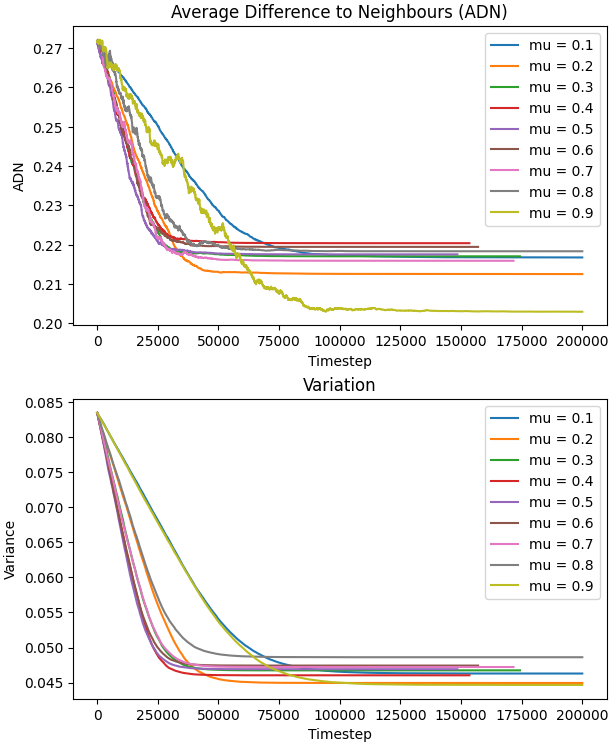
\includegraphics[width = 0.7\textwidth]{Images/Redone Images/diff mu values 2.png}
\caption{The average difference to neighbours (ADN) and variance as the lattice is iterated on. As this is a random process there will be some variation in the ADN and variance between $\mu$ values. $\mu$ values near 0.5 tend to reach equilibrium quicker than $\mu$ values near 0 and 1}
\end{figure}

A $\mu$ of 0.4 is used for discussion of other behaviors such as how the r value changes the system. This is done to set a standard between different lattices and to also ensure less iterations are necessary to achieve steady state. This behavior for the $\mu$ is also reflected in the literature, it was expected to have little impact on long term iterations of the lattice and the findings of this report support  this idea.

Another feature that doesn't affect the measurement outcomes is the dimensions of the lattice (assuming extremely small dimensions such as 1x1 or 2x2 lattices are not used). Assuming sufficiently large lattices, the amount of time steps to reach steady state increases, but the behavior at steady state does not change. This mimics how $\mu$ doesn't necessarily change the long term behavior, simply how long it takes to see this long term behavior. This is both for square lattices (which will be used as a baseline throughout the discussion) and for rectangular lattices. Clearly a differently-sized lattice will affect the area of clusters and the total number of clusters as there are more sites, but the behaviour of the phase transition (which will be discussed later) is almost identical as shown below. It appears that the area and number of clusters scales linearly with the size (or area specifically) of the lattice, which is unsurprising considering how this system is supposed to be scalable. Variance and ADN appear almost identical as these are unaffected by areas, only local behaviours within the lattice.

\begin{figure}[H]
\centering
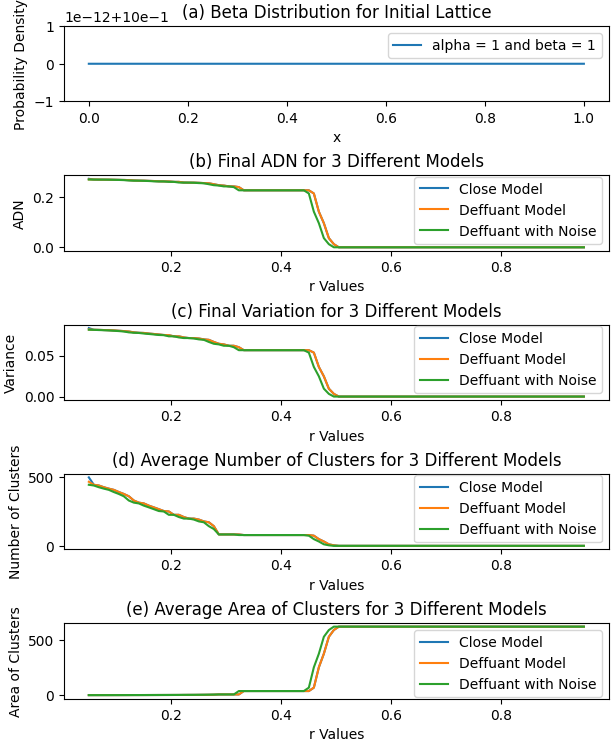
\includegraphics[width = 0.7\textwidth]{Images/Redone Images/x 25 y 25 alpha 1 beta 1 mu 04.png}
\caption{Various measurements on a 25 by 25 lattice. The lattice was run through the iteration process 20 separate times (or 20 different simulations as they will be referred to) and then measurements were averaged over those simulations. $\mu = 0.4$ was used for iteration. (a) The beta distribution used to generate the lattice. Using $\alpha = 1$ and $\beta = 1$ results in a uniform distribution for the generation of the lattice.
(b) The averaged ADN for the three models at the last iteration over different r values.
(c) The average variation for the three models at the last iteration over different r values.
(d) The average number of clusters for the three models at the last iteration over different r values.
(e) The average area of the clusters for the three models at the last iteration over different r values.}
\end{figure}

\begin{figure}[H]
\centering
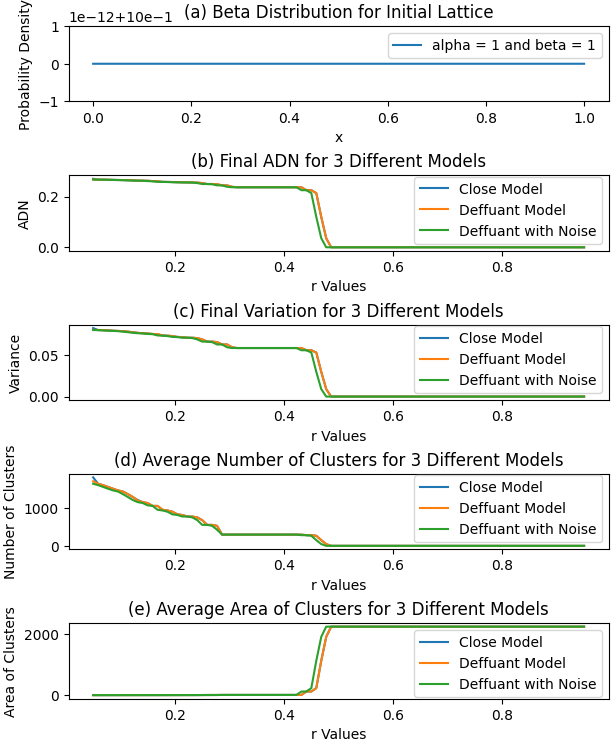
\includegraphics[width = 0.7\textwidth]{Images/Redone Images/x 30 y 75 alpha 1 beta 1 mu 04.png}
\caption{Various measurements on a 30 by 75 lattice. The lattice was run through the iteration process 20 separate times (or 20 different simulations as they will be referred to) and then measurements were averaged over those simulations. $\mu = 0.4$ was used for iteration. (a) The beta distribution used to generate the lattice. Using $\alpha = 1$ and $\beta = 1$ results in a uniform distribution for the generation of the lattice.
(b) The averaged ADN for the three models at the last iteration over different r values.
(c) The average variation for the three models at the last iteration over different r values.
(d) The average number of clusters for the three models at the last iteration over different r values.
(e) The average area of the clusters for the three models at the last iteration over different r values.}
\end{figure}

\begin{figure}[H]
\centering
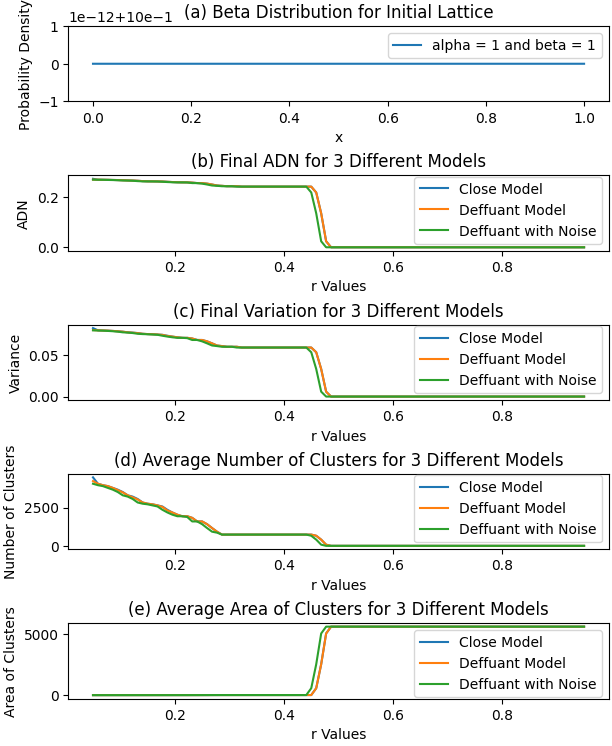
\includegraphics[width = 0.7\textwidth]{Images/Redone Images/x75 y 75 alpha 1 beta 1 mu 04.png}
\caption{Various measurements on a 75 by 75 lattice. The lattice was run through the iteration process 20 separate times (or 20 different simulations as they will be referred to) and then measurements were averaged over those simulations. $\mu = 0.4$ was used for iteration. (a) The beta distribution used to generate the lattice. Using $\alpha = 1$ and $\beta = 1$ results in a uniform distribution for the generation of the lattice.
(b) The averaged ADN for the three models at the last iteration over different r values.
(c) The average variation for the three models at the last iteration over different r values.
(d) The average number of clusters for the three models at the last iteration over different r values.
(e) The average area of the clusters for the three models at the last iteration over different r values.}
\end{figure}

It is clear however from the above that there is a difference between how the noisy Deffuant model behaves compared to the close Deffuant model and the normal Deffuant model. As this mostly pertains to the phase transition however it will not be discussed here.

\section{Cluster Behavior}
There are two regimes to consider, one regime where the r value for the update rule is below the phase transition and one where the r value is above. The phase transition will be discussed later.

\subsection{r Values Below Phase Transition}
For lower r values below the phase transition r value, the lattice sites will tend to a finite number of values based on the r value specified. This was previously given the name NVC.

\begin{figure}[H]
\centering
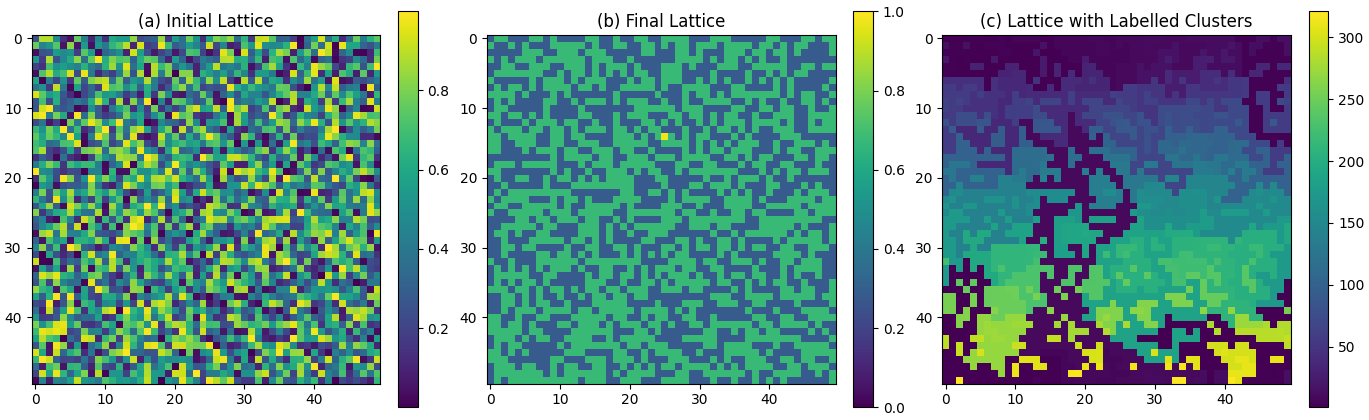
\includegraphics[width = 0.8\textwidth]{Images/labelled clust alpha 1 beta 1 mu 04 r 025.png}
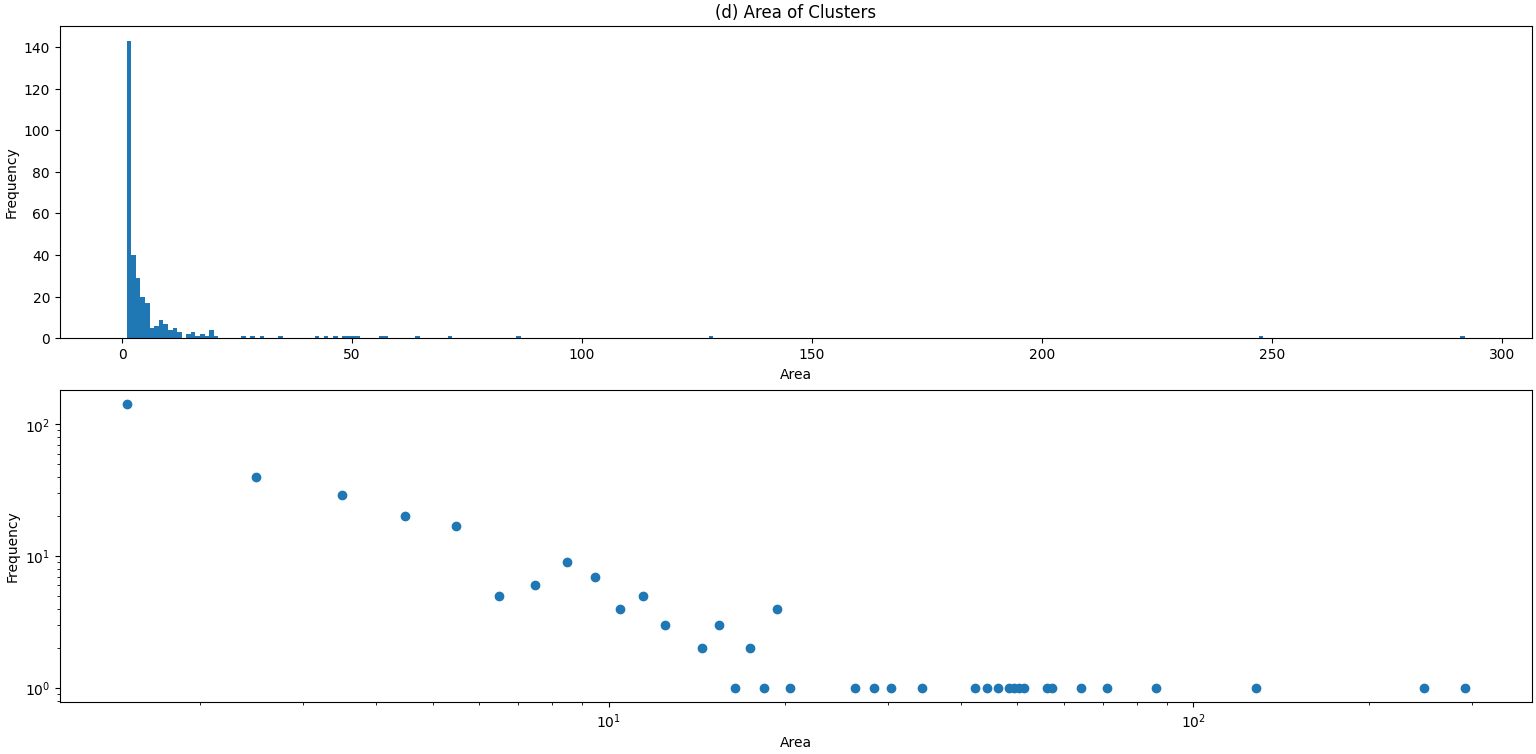
\includegraphics[width = 0.8\textwidth]{Images/area clust alpha 1 beta 1 mu 04 r 025.png}
\caption{(a) The initial lattice was generated with $\alpha = 1$ and $\beta = 1$.
(b) The lattice was iterated through using the Deffuant model with $\mu = 0.4$ and $r = 0.25$.
(c) The lattice with site values being the label of the cluster the site is a part of.
(d) The area of the cluster(s) as both a histogram and a log-log scatterplot.}
\end{figure}

It is worth noting that while the figure above may look like it only has two major values that the lattice sites take, there are other ones that are around 0.5, hence the use of NVC to try and capture these sites. Typically below the phase transition, all models follow NCV approximately well and as such one can approximate the long term behaviour for r values lower than the phase transition threshold. This is only approximate however and based on observation, it is not as certain as the behaviour above the phase transition threshold. Regardless, for lower r values the lattice always exhibits this splitting of lattice site values, regardless of $\mu$ values (assuming $\mu$ is not an extreme value like 0 or 1) and assuming the lattice generated uses a symmetric beta distribution (such as $\alpha = 0.5$ and $\beta = 0.5$).

For a lattice that is generated from an asymmetric beta distribution, the lattice reaches consensus with dots of lattice sites that cannot reach consensus.

\begin{figure}[H]
\centering
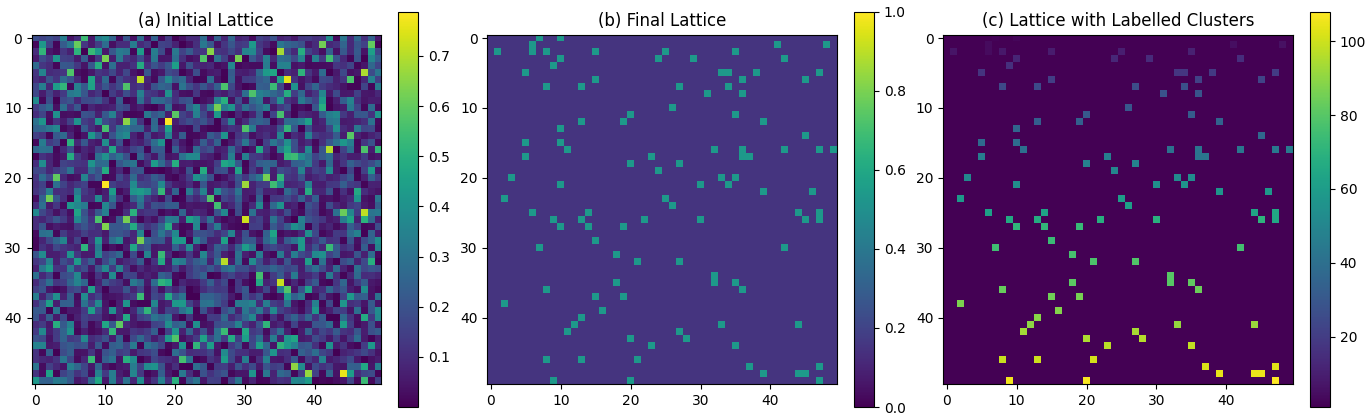
\includegraphics[width = 0.8\textwidth]{Images/labelled clust alpha 1 beta 5 mu 04 r 025.png}
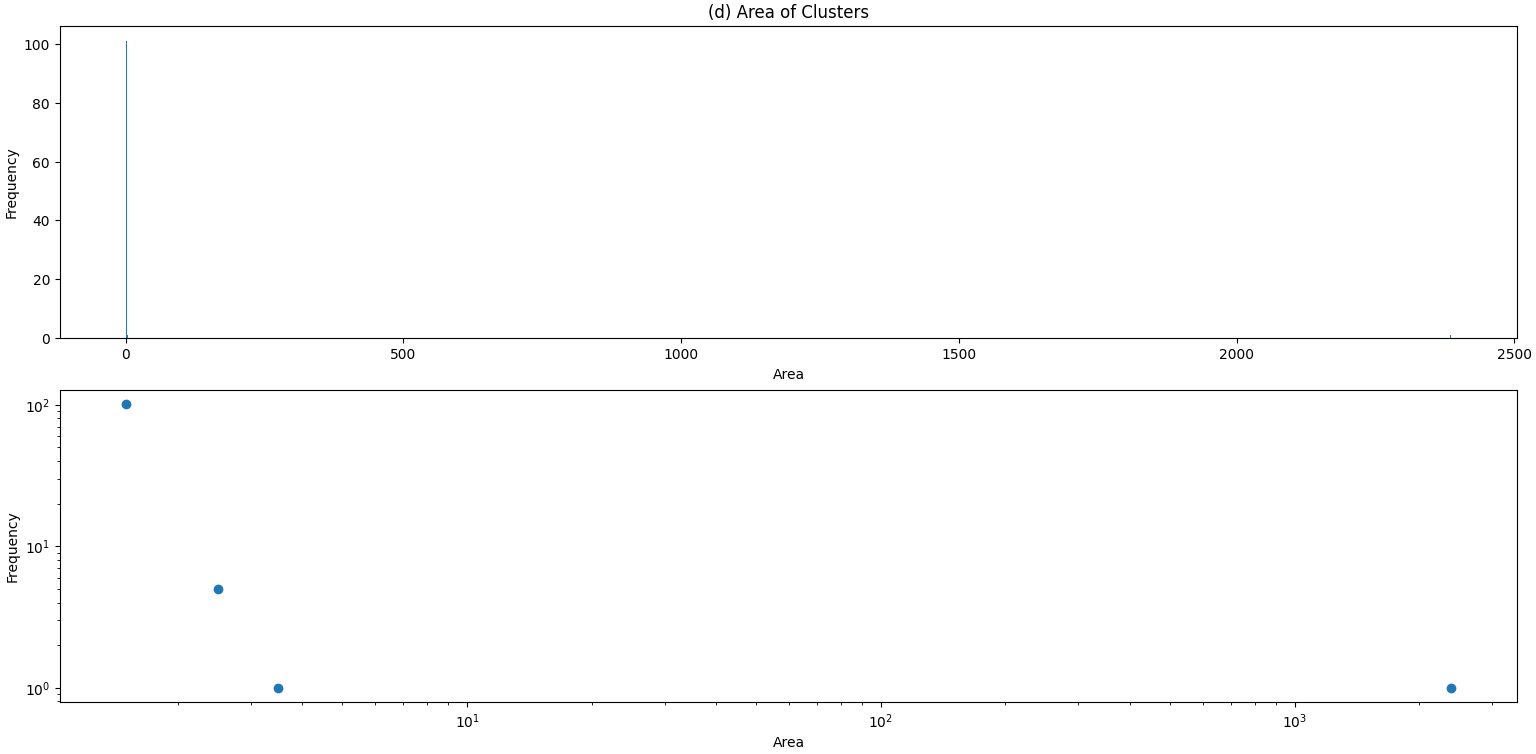
\includegraphics[width = 0.8\textwidth]{Images/area clust alpha 1 beta 5 mu 04 r 025.png}
\caption{(a) The initial lattice was generated with $\alpha = 1$ and $\beta = 5$.
(b) The lattice was iterated through using the Deffuant model with $\mu = 0.4$ and $r = 0.25$.
(c) The lattice with site values being the label of the cluster the site is a part of.
(d) The area of the cluster(s) as both a histogram and a log-log scatterplot.}
\end{figure}

Perhaps unsurprisingly, if the lattice is already dominated by one side of the bound, that domination will be reflected as the lattice is iterated on. Since there will be some values generated outside of the dominating values (at a much lower rate), those lattice site values will not be able to communicate with the majority, causing spots that do not agree with the majority of the lattice, hence the spotty iterated lattice.

The number of clusters trends downwards as r increases towards the phase transition. As r increases, more lattice sites are able to communicate with each other, resulting in the values the lattice sites can take decreasing and therefore the number of clusters also trends downwards.

\subsection{r Values Above Phase Transition}
For higher r values above the phase transition, the lattice tends to reach consensus. This occurs for the close Deffuant model, Deffuant model and noisy Deffuant model, assuming that the r value is larger than the phase transition r value.

\begin{figure}[H]
\centering
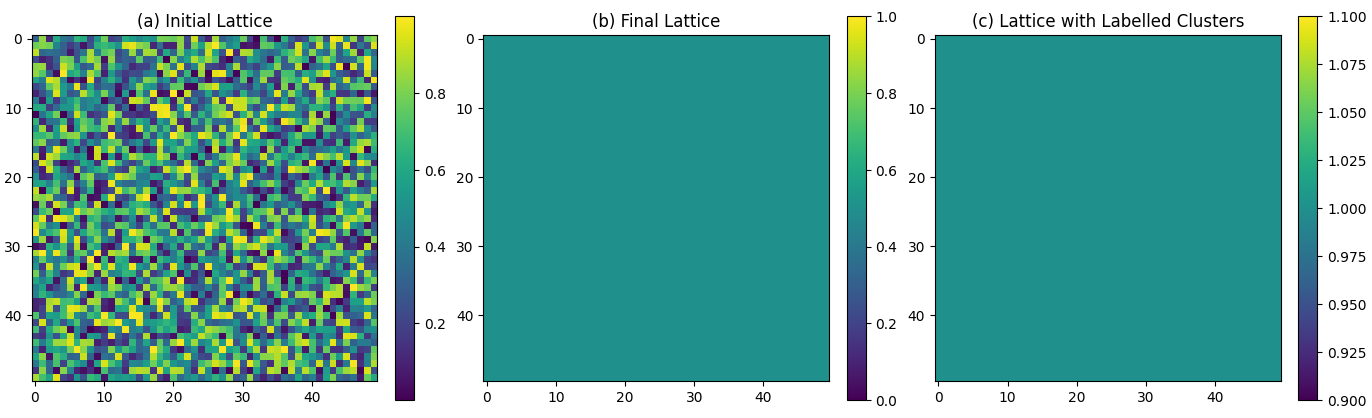
\includegraphics[width = 0.8\textwidth]{Images/labelled clust alpha 1 beta 1 mu 04 r 08.png}
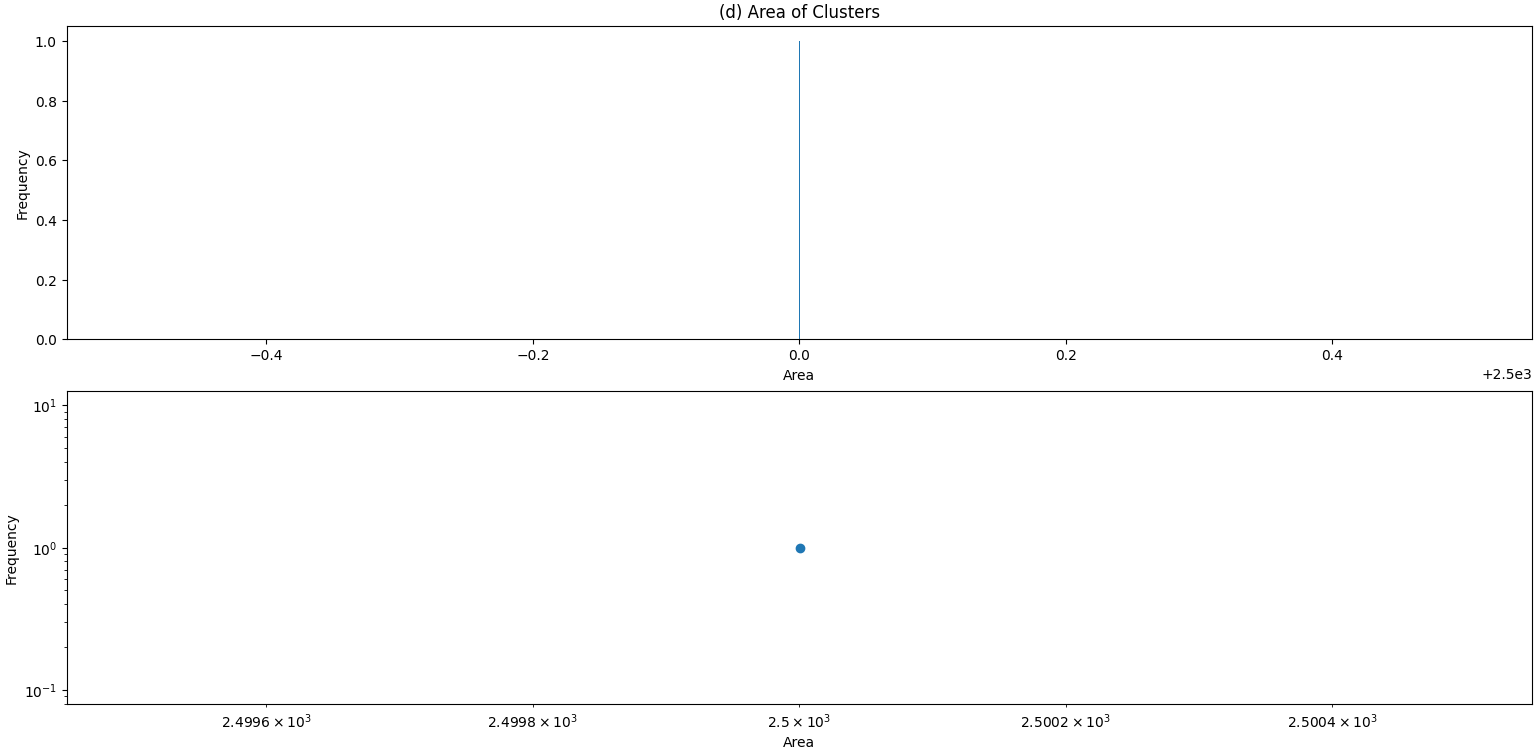
\includegraphics[width = 0.8\textwidth]{Images/area clust alpha 1 beta 1 mu 04 r 08.png}
\caption{(a) The initial lattice was generated with $\alpha = 1$ and $\beta = 1$.
(b) The lattice was iterated through using the Deffuant model with $\mu = 0.4$ and $r = 0.8$.
(c) The lattice with site values being the label of the cluster the site is a part of.
(d) The area of the cluster(s) as both a histogram and a log-log scatterplot.}
\end{figure}

From the above figure, one can see that it approaches consensus with all sites being extremely close in value to each other to the point of forming on large "cluster" (although the word "cluster" loses meaning in this case as its just one value for the whole lattice). This happens practically every time for large enough r value and as such the exact long term behaviour is a lot more predictable than that for low r values.

\section{Phase Transition}
Literature states that a phase transition for a network/lattice occurs at $r=0.5$ \cite{FORTUNATO_2004} \cite{lanchier2023deffuantopiniondynamicsattraction}, where if $r<0.5$ the system approaches clustering behaviors and if $r>0.5$ the system approaches consensus among the agents. The simulations tends to agree with this assessment for a uniform distribution within the starting lattice.

\begin{figure}[H]
\centering
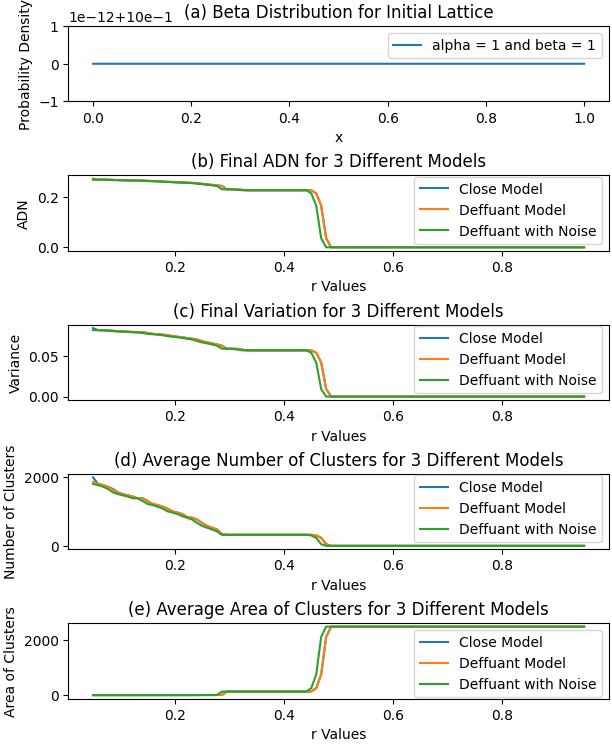
\includegraphics[width=0.7\textwidth]{Images/Redone Images/alpha 1 beta 1 mu 04.png}
\caption{Various measurements on a 50 by 50 lattice. The lattice was run through the iteration process 20 separate times (or 20 different simulations as they will be referred to) and then measurements were averaged over those simulations. $\mu = 0.4$ was used for iteration. (a) The beta distribution used to generate the lattice. Using $\alpha = 1$ and $\beta = 1$ results in a uniform distribution for the generation of the lattice.
(b) The averaged ADN for the three models at the last iteration over different r values.
(c) The average variation for the three models at the last iteration over different r values.
(d) The average number of clusters for the three models at the last iteration over different r values.
(e) The average area of the clusters for the three models at the last iteration over different r values.}
\end{figure}

From the above the phase transition appears to occur at approximately $r = 0.5$ for the close Deffuant model and the normal Deffuant model, however the phase transition occurs slightly earlier for the noisy Deffuant model. This also occurs for other initial lattices that use a beta distribution for generation that is symmetrical around 0.5, as shown below.

\begin{figure}[H]
\centering
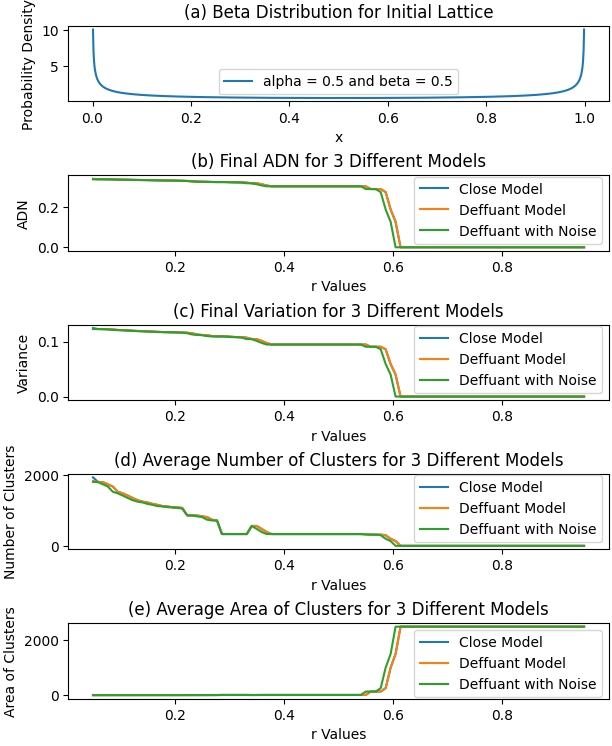
\includegraphics[width = 0.7\textwidth]{Images/Redone Images/alpha 05 beta 05 mu 04.png}
\caption{Various measurements on a 50 by 50 lattice. The lattice was run through the iteration process 20 separate times (or 20 different simulations as they will be referred to) and then measurements were averaged over those simulations. $\mu = 0.4$ was used for iteration. (a) The beta distribution used to generate the lattice. Using $\alpha = 0.5$ and $\beta = 0.5$ results in a more polarised distribution for the generation of the lattice.
(b) The averaged ADN for the three models at the last iteration over different r values.
(c) The average variation for the three models at the last iteration over different r values.
(d) The average number of clusters for the three models at the last iteration over different r values.
(e) The average area of the clusters for the three models at the last iteration over different r values.}
\label{alp_05_bet_05}
\end{figure}

\begin{figure}[H]
\centering
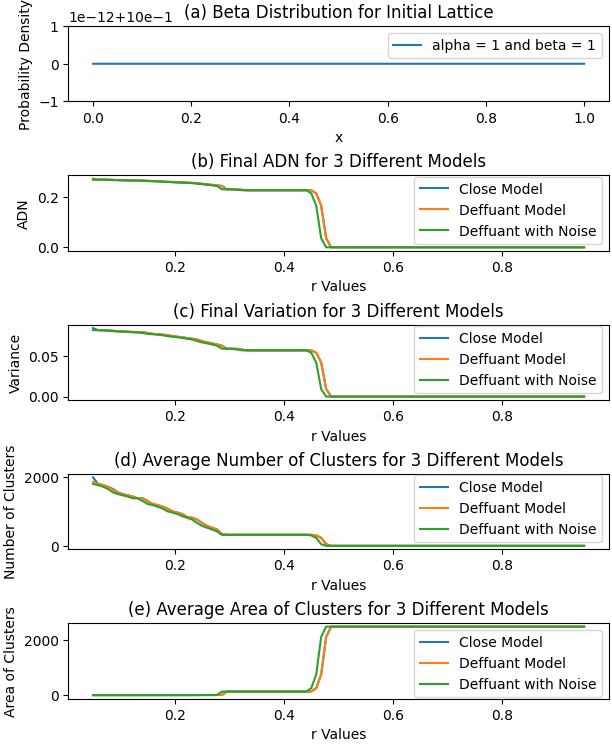
\includegraphics[width = 0.7\textwidth]{Images/Redone Images/alpha 1 beta 1 mu 04.png}
\caption{Various measurements on a 50 by 50 lattice. The lattice was run through the iteration process 20 separate times (or 20 different simulations as they will be referred to) and then measurements were averaged over those simulations. $\mu = 0.4$ was used for iteration. (a) The beta distribution used to generate the lattice. Using $\alpha = 1$ and $\beta = 1$ results in a uniform distribution for the generation of the lattice.
(b) The averaged ADN for the three models at the last iteration over different r values.
(c) The average variation for the three models at the last iteration over different r values.
(d) The average number of clusters for the three models at the last iteration over different r values.
(e) The average area of the clusters for the three models at the last iteration over different r values.}
\end{figure}

\begin{figure}[H]
\centering
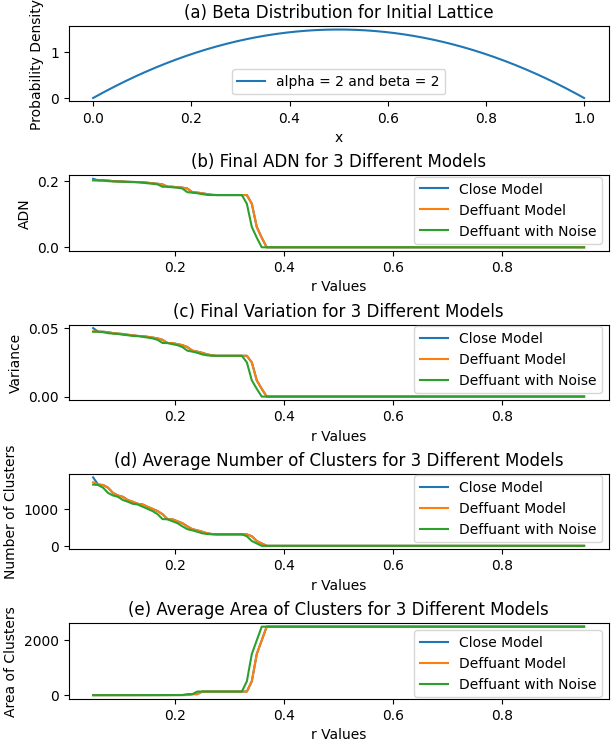
\includegraphics[width = 0.7\textwidth]{Images/Redone Images/alpha 2 beta 2 mu 04.png}
\caption{Various measurements on a 50 by 50 lattice. The lattice was run through the iteration process 20 separate times (or 20 different simulations as they will be referred to) and then measurements were averaged over those simulations. $\mu = 0.4$ was used for iteration. (a) The beta distribution used to generate the lattice. Using $\alpha = 2$ and $\beta = 2$ results in a more centralised distribution for the generation of the lattice.
(b) The averaged ADN for the three models at the last iteration over different r values.
(c) The average variation for the three models at the last iteration over different r values.
(d) The average number of clusters for the three models at the last iteration over different r values.
(e) The average area of the clusters for the three models at the last iteration over different r values.}
\end{figure}

While this behaviour is very clear in the case where the beta distribution used to generate the initial lattice is symmetric around 0.5, it is less clear with an asymmetric beta distribution, although it still appears to exhibit the same behaviour.

\begin{figure}[H]
\centering
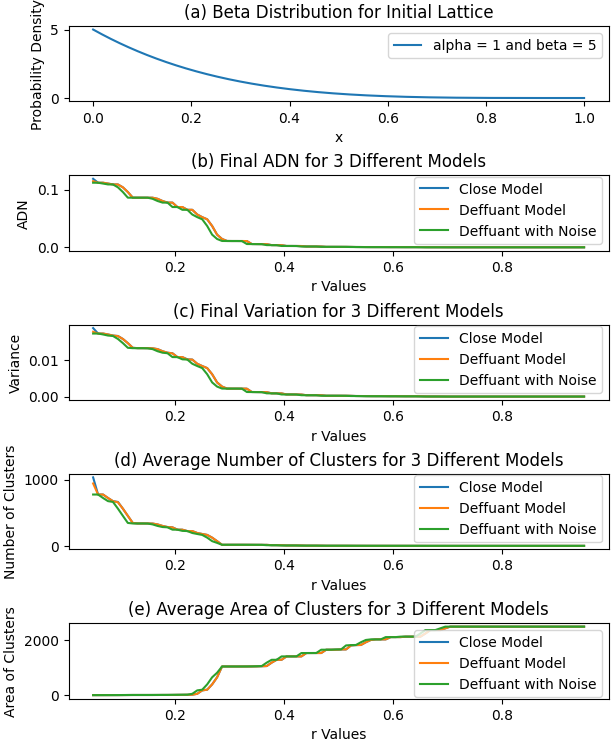
\includegraphics[width = 0.7\textwidth]{Images/Redone Images/alpha 1 beta 5 mu 04.png}
\caption{Various measurements on a 50 by 50 lattice. The lattice was run through the iteration process 20 separate times (or 20 different simulations as they will be referred to) and then measurements were averaged over those simulations. $\mu = 0.4$ was used for iteration. (a) The beta distribution used to generate the lattice. Using $\alpha = 1$ and $\beta = 5$ results in a distribution that skwes towards 0 for the generation of the lattice.
(b) The averaged ADN for the three models at the last iteration over different r values.
(c) The average variation for the three models at the last iteration over different r values.
(d) The average number of clusters for the three models at the last iteration over different r values.
(e) The average area of the clusters for the three models at the last iteration over different r values.}
\end{figure}

\begin{figure}[H]
\centering
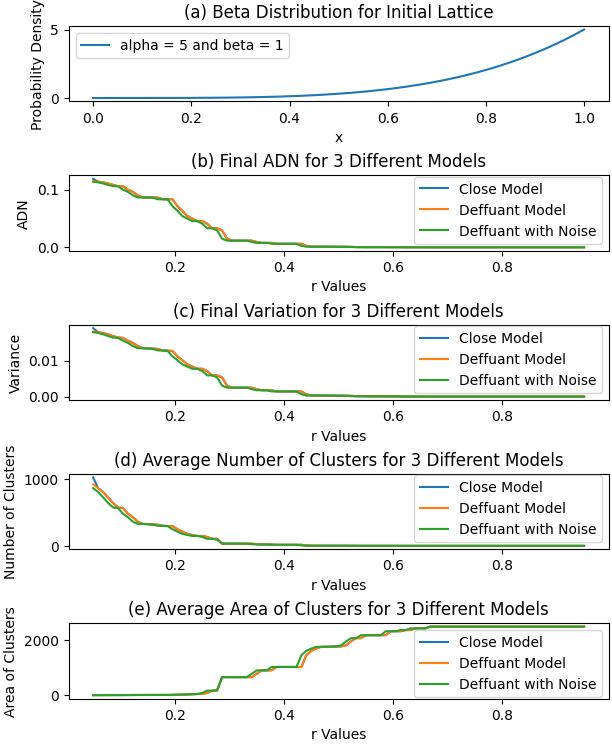
\includegraphics[width = 0.7\textwidth]{Images/Redone Images/alpha 5 beta 1 mu 04.png}
\caption{Various measurements on a 50 by 50 lattice. The lattice was run through the iteration process 20 separate times (or 20 different simulations as they will be referred to) and then measurements were averaged over those simulations. $\mu = 0.4$ was used for iteration. (a) The beta distribution used to generate the lattice. Using $\alpha = 5$ and $\beta = 1$ results in a distribution that skews towards 1 for the generation of the lattice.
(b) The averaged ADN for the three models at the last iteration over different r values.
(c) The average variation for the three models at the last iteration over different r values.
(d) The average number of clusters for the three models at the last iteration over different r values.
(e) The average area of the clusters for the three models at the last iteration over different r values.}
\end{figure}

This behaviour occurs due to how the system typically reaches equilibrium. For low r values (r values below the phase transition point), the system will organise itself such that sites only take a finite number of values. Take the example from section 2.4, where a value of $r = 0.25$ results in the lattice sites taking one of three distinct values. An example run using the normal Deffuant model is shown below of this situation.

\begin{figure}[H]
\centering
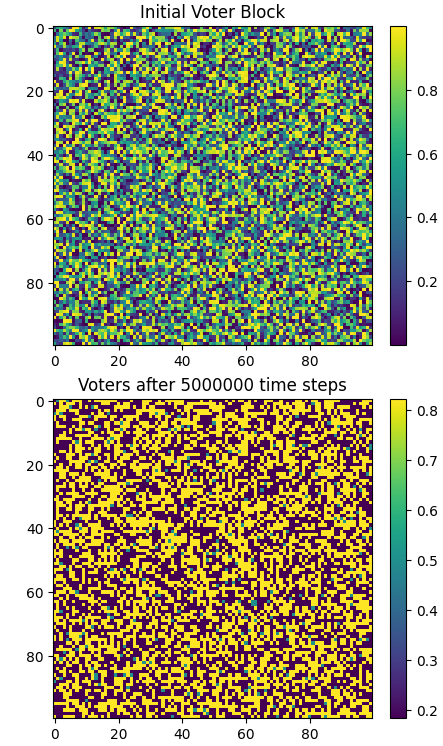
\includegraphics[width=0.7\textwidth]{Images/x 100 y 100 r 025 mu 04 deff lat gen.png}
\caption{The sites in the lattice have one of 3 values, 0.184, 0.503 and 0.821. Initial lattice has $\alpha = 0.5$ and $\beta = 0.5$ for beta distribution generation, dimensions of 100x100 and the model used is the normal Deffuant model with a $\mu$ value of $\mu = 0.4$.}
\end{figure}

From the above, one can see that the magnitude of the difference between 0.184 and 0.503 is greater than 0.25 and likewise for 0.503 and 0.184 and 0.821. So while the system is in the process of reaching equilibrium, values within 0.25 of 0.184, 0.503 or 0.821 will approach those respective values, but cannot reach other values via communication. This is all because $r=0.25$ in this case. Once r is sufficiently large however, all sites are able to communicate with each other, they may need to communicate with other sites closer in value first but they eventually are able to be influenced by any and all sites and due to the updating rule they will eventually converge to consensus. The value of r this typically happens at is $r = 0.5$ (for uniform starting lattice), as enough sites are able to communicate for consensus. However, with the noisy Deffuant model, r is not limited to being a single value, it has a chance to either be slightly less than or (more importantly for the phase transition) greater than a mean value. Typically the variation from the mean was made small, so the noisy Deffuant model mostly followed the other two models for most r values. Near the phase transition however, the spread allows r to take values that go over the typical phase transition value. If this occurs enough, the system behaves as if it is over the phase transition value of r, and so the system transitions to consensus earlier than the other two models. The reason it occurs earlier is because consensus cannot be undone between sites due to how the update rule always brings the value of the two sites closer, the update rule cannot take two sites' values further apart.

One may have also noticed that the phase transition is affected by the initial beta distribution used to generate the lattice. If the distribution used is more central, the phase transition occurs for a smaller r value and if the distribution is more extreme on opposite ends (which will be referred to as the extreme case) then the phase transition occurs for a higher r value, as seen in Figure \ref{alp_05_bet_05}. For the extreme case, the lattice sites will remain extreme as there are little central sites within range r to help bridge the gap between the extremes. This results in the r value for the phase transition increasing as it needs to be sufficiently large to bridge the two extremes directly, rather than having central sites to "connect" the two extremes. A more central distribution for the initial lattice results in a phase transition at a lower r value as the larger central population brings the more extreme lattice sites closer to central values (assuming the range r at which is large enough to capture some of the extreme sites), and as the central sites greatly outnumber the extreme sites, the central sites end up dominating. This causes consensus for lower r values.

\section{Conclusion}
This implementation of the Deffuant model to a square/rectangular periodic lattice supports the findings of the literatures' conclusions. The phase transition r value is about 0.5 for a uniform lattice using the Deffuant model, as well as for the close Deffuant model. The noisy Deffuant model consistently has a phase transition point lower than that of the other two models. $\mu$ values and the size of the lattice (assuming large enough) had little effect on the long term behaviour of the phase transition, instead affecting the number of iterations needed to reach an equilibrium. Above the phase transition, the long term behaviour of the lattice is for it to reach consensus. Below the phase transition, the lattice tended to have lattice sites go to a finite number of values, dependent on the r value. For symmetric but non-uniform probability of values in the starting lattice, the phase transition would either be less than 0.5 (for more centralised distribution) or greater than 0.5 (for more polarised distribution) in the long term. Asymmetric distributions do not seem to exhibit a phase transition like the symmetric distributions do.